\section{Asuro}
\subsection{Aufbau}
\begin{frame}[c]
	\frametitle{\currentsection}
	\framesubtitle{\currentsubsection}
	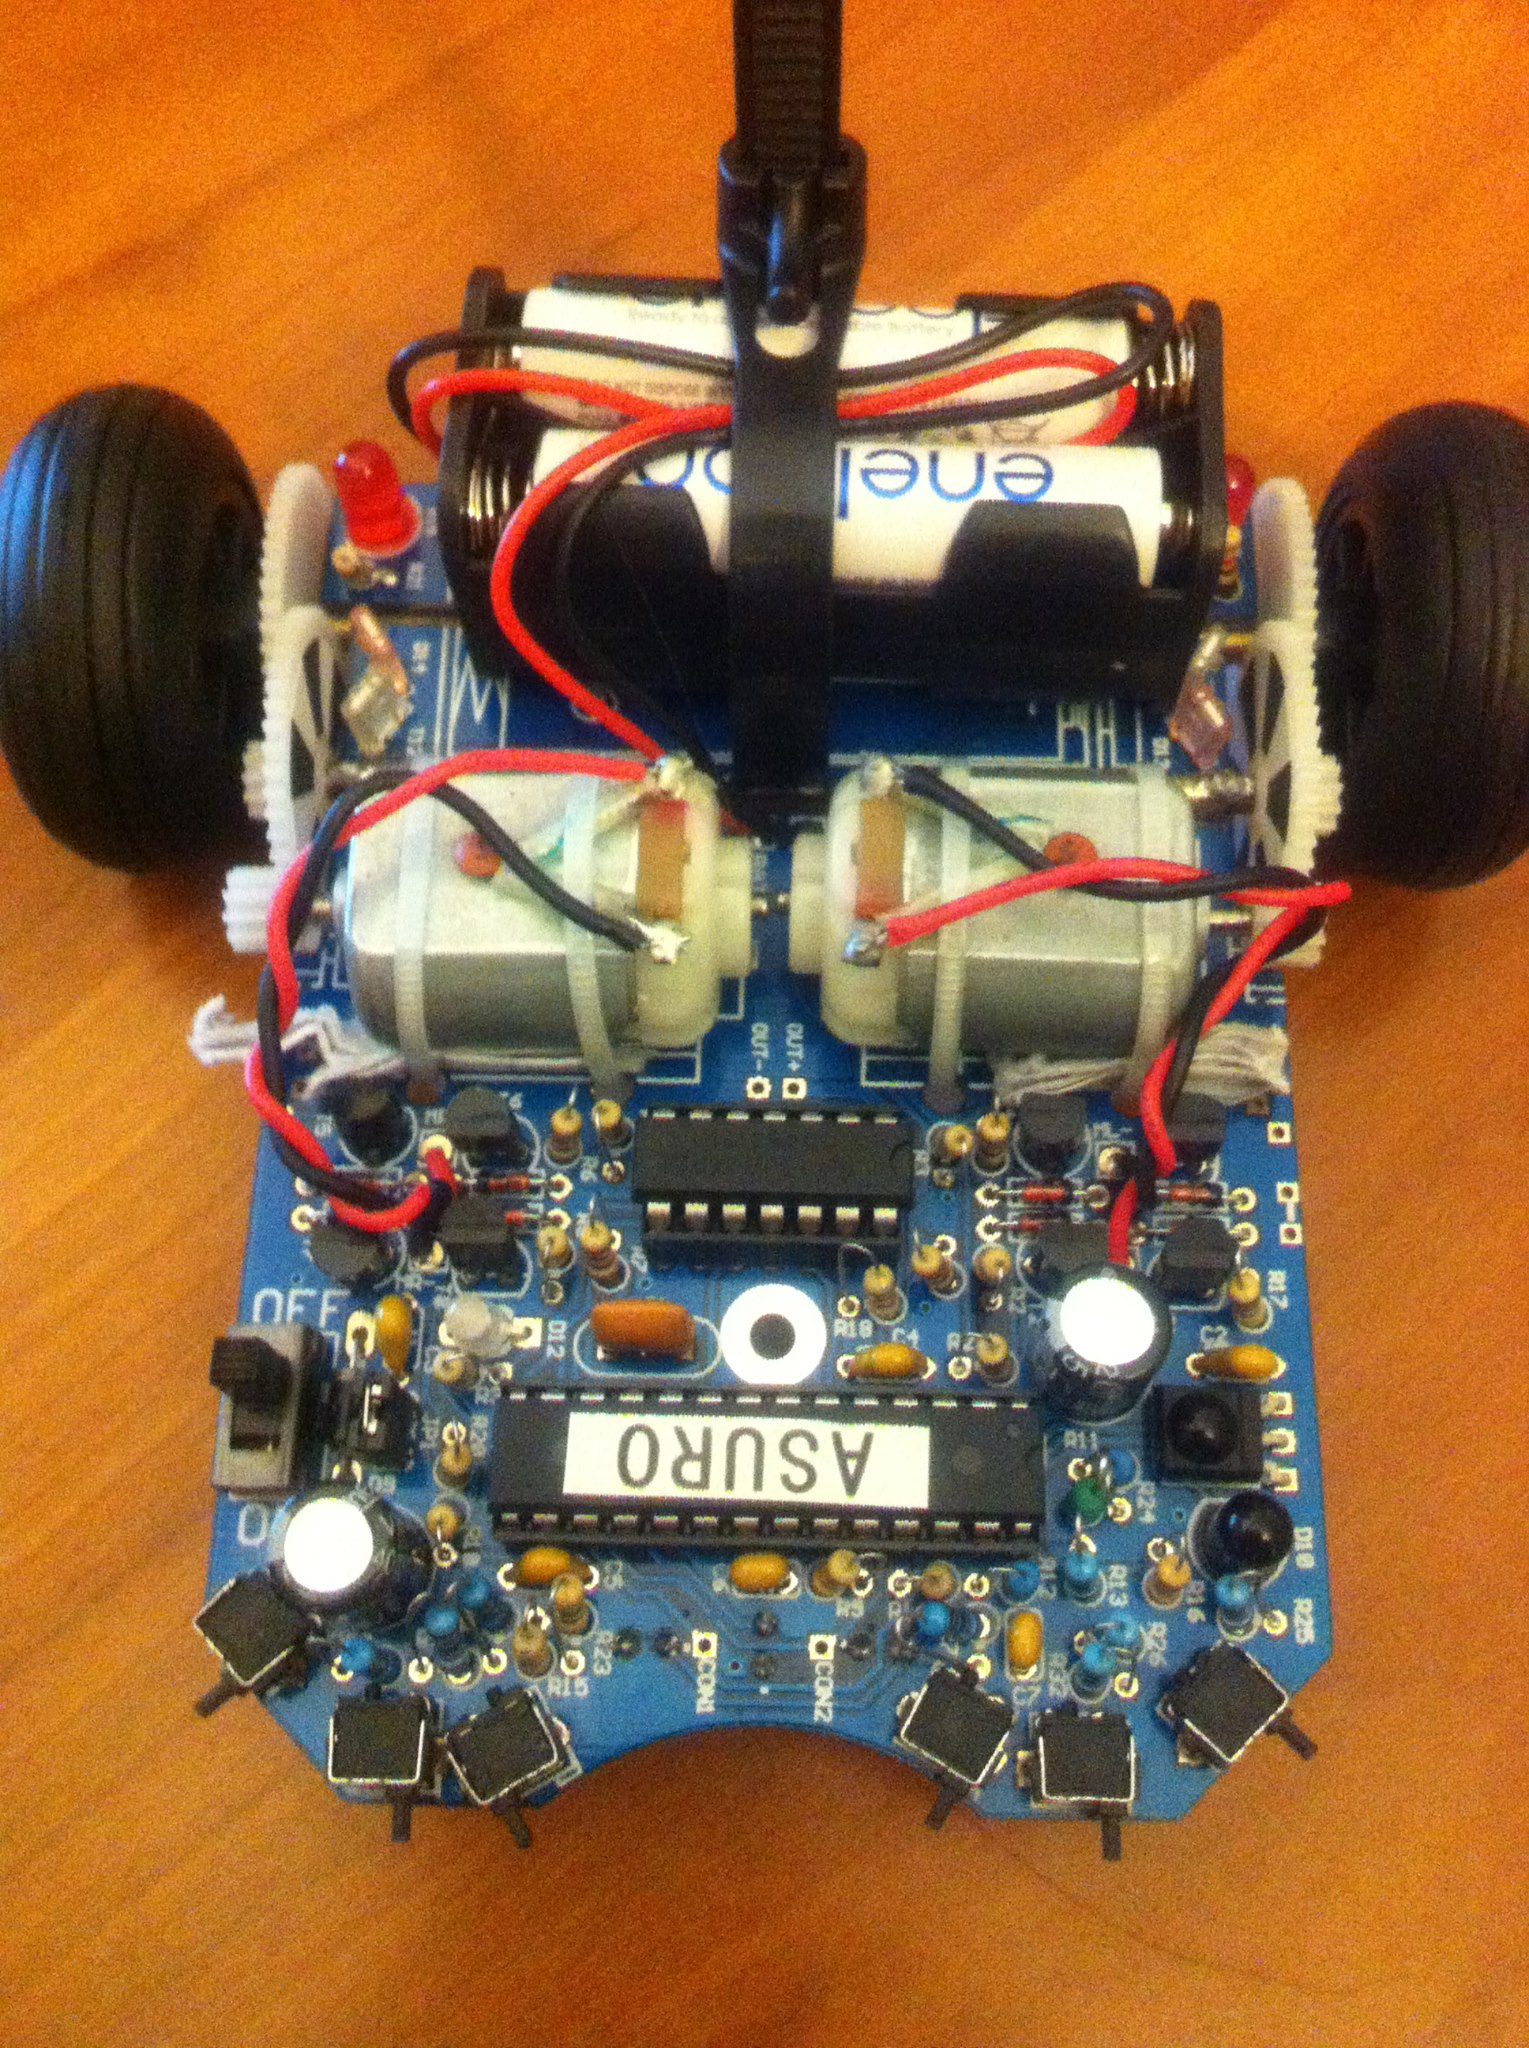
\includegraphics[scale=0.125, angle=90, origin=c]{Bilder/asuro_top}
\end{frame}
\begin{frame}[c]
	\frametitle{\currentsection}
	\framesubtitle{\currentsubsection}
	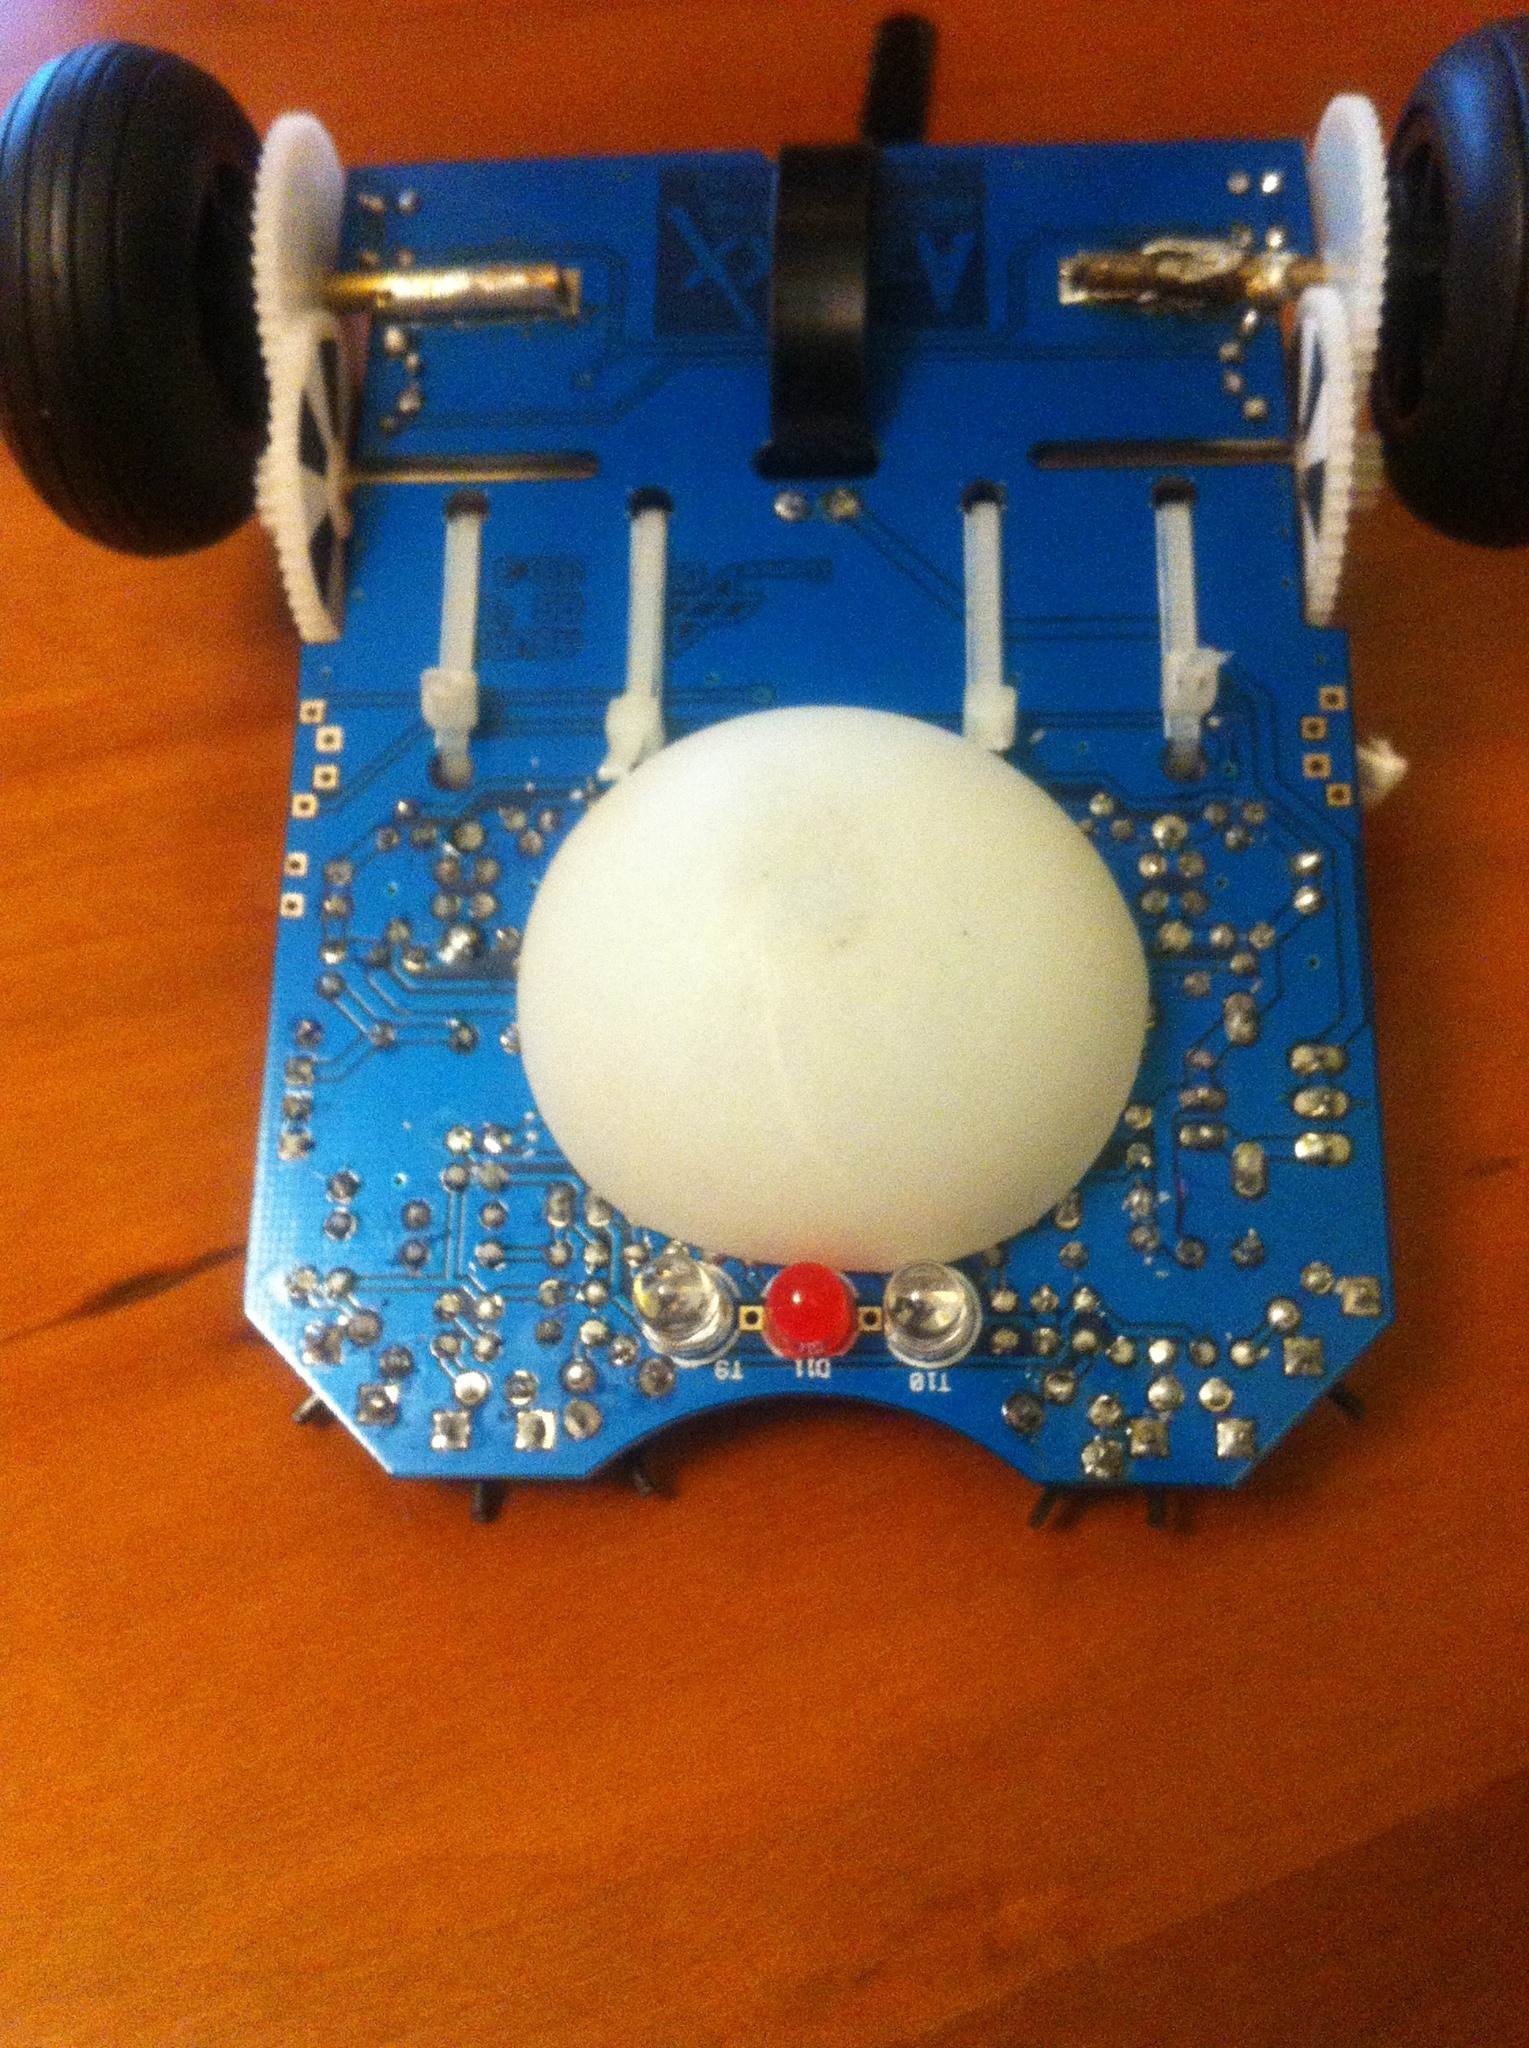
\includegraphics[scale=0.125, angle=90, origin=c]{Bilder/asuro_bottom}
\end{frame}


\subsection{Library}
\begin{frame}[c]
	\frametitle{\currentsection}
	\framesubtitle{\currentsubsection}
	\begin{block}<1->{Wichtige Funktionen}
		\begin{itemize}
			\item void Init();
			\item void GoTurn(int16\_t distance, int16\_t degree, uint8\_t speed);
			\item void BackLED(const uint8\_t left, const uint8\_t right);
			\item void FrontLED(const uint8\_t status);
			\item void StatusLED(const uint8\_t color);
			\item void MotorDir(const uint8\_t left\_dir, const uint8\_t right\_dir);
			\item void MotorSpeed(const uint8\_t left\_speed, const uint8\_t right\_speed);
			\item void LineData(uint16\_t * const data);
			\item uint8\_t PollSwitch(void);
			\item void msleep(uint16\_t ms);
		\end{itemize}
	\end{block}
\end{frame}


\subsection{Beispiel Programm}
\begin{frame}[c]
	\frametitle{\currentsection}
	\framesubtitle{\currentsubsection}
	\lstinputlisting[language=C]{Code/Examples/example.c}
\end{frame}